\documentclass[letterpaper]{article}
\usepackage{iccc}

\usepackage{times}
\usepackage{helvet}
\usepackage{courier}
\usepackage{graphicx}
\usepackage[ruled]{algorithm2e}
\usepackage{amsmath}
\usepackage[T1]{fontenc}
\usepackage[hidelinks]{hyperref}
\urlstyle{same}
\usepackage[margin=0.5in]{geometry}

\pdfinfo{
/Title (Automatic Puzzle Level Generation: A General Approach using a Description Language)
/Subject (Proceedings of CCGW 2015)
/Author (Ahmed Khlifa, Magda Fayek)}
% The file iccc.sty is the style file for ICCC proceedings.
%
\title{Automatic Puzzle Level Generation:\\
A General Approach using a Description Language}
\author{Ahmed Khalifa \and Magda Fayek\\
Computer Engineering Department\\
Faculty of Engineering, Cairo University\\
Cairo University Road, Giza, Egypt\\
amidos2002@hotmail.com, magdafayek@ieee.org\\
}
\setcounter{secnumdepth}{0}

\newcommand{\chref}[1]{Chapter~\ref{Chapter:#1}}
\newcommand{\appref}[1]{Appendix~\ref{Appendix:#1}}
\newcommand{\secref}[1]{Section~\ref{Section:#1}}
\newcommand{\eqnref}[1]{Equation~\ref{Equation:#1}}
\newcommand{\tabref}[1]{Table~\ref{Table:#1}}
\newcommand{\figref}[1]{Figure~\ref{Figure:#1}}
\newcommand{\algref}[1]{Algorithm~\ref{Algorithm:#1}}
\setlength{\textfloatsep}{10pt}

\begin{document} 
\maketitle
\begin{abstract}
In this paper, we present a general technique to evaluate and generate puzzle levels made by Puzzle Script. Puzzle Script is a videogame description language for scripting puzzle games, which was created by Stephen Lavelle\cite{puzzleScript}. We propose a system to help in generating levels for Puzzle Script without any restriction on the rules. Two different approaches are used with a trade off between speed (Constructive approach) and playability (Genetic approach). These two approaches use a level evaluator that calculates the scores of the generated levels based on their playability and challenge. The generated levels are assessed by human players statistically, and the results show that the constructive approach is capable of generating playable levels up to 90\%, while genetic approach can reach up to 100\%. The results also show a high correlation between the system scores and the human scores.
\end{abstract}

\section{Introduction}
During the early days of Video Games, games were created by few people in their spare time. Most of the time was spent in programming the game, while a small portion was dedicated for graphics, sounds, and music because of the technical limitations of the devices at that time. Although these limitation are no more, game production still takes long time. Most of that time is spent on creating content for the game (graphics, music, sounds, levels, and ...etc)\cite{budgetAAA}; for example creating graphics for a huge main stream game may take hundreds of artist working for a year or two. That is why the production cost of a huge game reaches millions of dollars\cite{gameCost}.\\\par

This huge production cost is one of the reasons for using Procedural Content Generation(PCG). PCG means generating game content using a computer. It was first developed due to technical limitations (small disk space) and the need to provide a huge amount of content\cite{pcgFirstGame}. Although technical difficulties become history and storage is no longer a problem, PCG is still one of the hot topics in Video Games Industry and Research. PCG helps us reduce development time and cost, be creative, and understand the process of creating game content. PCG can be used to generate different game aspects for example Textures, Sounds, Music, Levels, Rules, and ...etc.\\\par

Level Generation is used to introduce a huge amount of levels that humans can not generate manually in a reasonable time. Level Generation has always been done for a specific game using lots of hacks to improve the output result. These hacks cause the output levels to follow certain guidelines which limit the amount of possible levels. On the other hand these guidelines ensure that output levels are all playable (can reach goal of the game) and satisfactory by all players\cite{mcGenerateEverything}.\\\par

In this paper, Our system utilizes small prior knowledge about Puzzle Script. This knowledge helps in generating playable and challenging levels without any restrictions or hacks.

\section{Background}
We can not generate general levels without having a methodology to describe the games. Video Game Description Language(VGDL) was originally invented to help on the work for General Video Game Playing(GVGP)\cite{gvgp} at Standford University. Puzzle Script(PS) is a VGDL created by Stephan Lavelle to help game designers and developers to create puzzle games\cite{puzzleScript}. Games generated by PS are time stepped games similar to Sokoban\cite{sokoban}.\\\par

PS file starts with some meta data like game name, author name, and website then it is divided into 7 sections objects, legend, sounds, collision layers, rules, win conditions, and levels. In this work, we focus on rules, win conditions, and levels sections. Rules are a set of production rules that govern how the game will be played. For example, \begin{center}[> Player | Crate] -> [> Player | > Crate]\end{center} means if there is a Player and Crate beside each other, and the Player moves towards the Crate, then both the Player and the Crate will move in the same direction. Win conditions are group of rules that identify when the level should end. Levels are 2D matrices showing the current configuration for each game level using objects identified in objects section.

\section{Literature Review}
As far as we know, no previous research was done in general puzzle level generation. Most of the previous work is done for a certain game. This section will show most previous work that was done in level generation. One of the earliest research in Puzzle Games was by Murase et al.\cite{sokobanLevelGenerationOld}. Murase et al. work focused on generating well designed solvable levels for Sokoban\cite{sokoban}. Breadth First Search(BFS) is used to check playability. Results show that for every 500 generated levels only 14 are considered as good levels. These levels are characterized by having a short solution sequence. Taylor and Parberry\cite{sokobanLevelGenerationNew} followed Yoshio Murase et al. work\cite{sokobanLevelGenerationOld} to improve generated level quality. Their system places the crates at the farthest possible location from the target using a similar algorithm to BFS. The generated levels are not suffering from the problem of short solution sequences presented in Yoshio Murase et al. work\cite{sokobanLevelGenerationOld}.\\\par

Rychnovsky\cite{fruitDatingPCG} work focused on generating levels for his new game Fruit Dating\cite{fruitDating}. Rychnovsky developed a level editor that can be used to generate new levels or test playability of certain level. Generating new levels is done by generating level layout and placing game objects in certain locations based on some prior game knowledge, then check for a solution using a similar algorithm to BFS. The technique doesn't take more than couple of minutes to generate a level with no direct way to influence difficulty in the generated levels.\\\par

Shaker et al.\cite{ctrAutomaticGeneration} worked on generating levels for physics based puzzle games. They applied their technique on Cut The Rope(CTR)\cite{cutTheRope}. Shaker et al. used Grammar Evolution (GE) technique to generate levels for CTR. The grammar is designed to ensure that every game object appears at least one time. The fitness function depends on some heuristic measures based on prior knowledge about the game and the result of several playouts using a random player. Shaker et al. generated 100 playable levels and analyzed them according to some metrics such as frequency, density, and ...etc. Shaker et al.\cite{ctrSimulationApproach} conducted their research on CTR to improve generated level quality. They replaced the random player with an intelligent one. The generated levels are far more diverse because the random player discards some potential levels in the search space.\\\par

Shaker et al.\cite{ctrProgressiveApproach} introduced a new generation technique named Progressive Approach. It can be used on any kind of games to reduce the generation time. Progressive Approach starts by using GE to generate a time-line of game events, then an intelligent player is used to map and evaluate the time-line to a playable level. Shaker et al. tested the new technique on CTR and compared its results with their previous work\cite{ctrSimulationApproach}. The results indicates a huge decrease in generation time, but the quality of the levels depended on the mapping process of the intelligent player.\\\par

Smith et al.\cite{refractionStudy} worked on generating puzzle levels for Refraction\cite{refraction}. The system starts by generating a solution outline, followed by translating the outline into a geometric layout, then testing the generated level for playability. Smith et al. implemented the system using two different ways (Algorithmic approach and Answer Set Programming (ASP)). Results shows that ASP is faster than Algorithmic approach, while Algorithmic approach produces more diverse levels than ASP.

\section{Methodology}
Level Generation is not an easy task specially when the game rules are not known before generation. Although some of the previous research suggested a general technique to generate levels, it is still based on designing a game specific fitness function. Our approach relies heavily on the understanding of the current game rules and some prior knowledge about Puzzle Script language. \figref{levelGenBlockDiagram} shows a high level block diagram of the system.\\\par

\begin{figure*}[ht]
  	\centering
    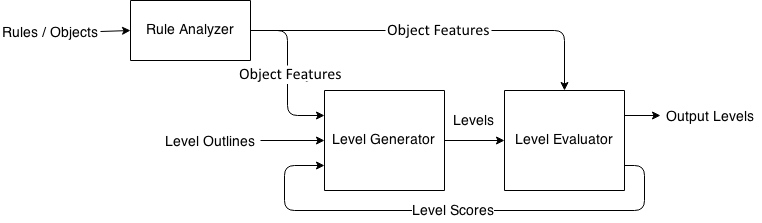
\includegraphics[width=0.9\textwidth]{Images/levelGenBlockDiagram}
    \caption{High level system block diagram for Level Generation}
    \label{Figure:levelGenBlockDiagram}
\end{figure*}

The system starts by analyzing the current game rules using a Rule Analyzer. The output of the Rule Analyzer and the Level Outlines are fed to a Level Generator. The Level Generator generates some initial level layouts using Genetic Algorithm(GA) or Constructive Algorithm(CA). The generated levels are subjected to a Level Evaluator. The Level Evaluator measures their playability and challenge using an automated player. The following subsections will describe each of these steps in details.

\subsection{Rule Analyzer}
The Rule Analyzer is the first module in our system. It analyzes game rules and extract some useful information about each object. The extracted information is fed to the Level Generator and the Level Evaluator. The extracted information for each object are:
\begin{itemize}
	\item \emph{Type:} Object type depends on its presence in the Puzzle Script file. There are 4 different types:
	\begin{itemize}
		\item \emph{Rule Object:} Any object that appears in a rule is defined as a rule object.
		\item \emph{Player Object:} It is main game object and it is defined by name "Player" in the Puzzle Script.
		\item \emph{Winning Object:} They are objects appearing in the winning condition.
		\item \emph{Solid Object:} All objects that does not appear in any rule but on the same collision layer with a Rule Object.
	\end{itemize}
	\item \emph{Subtype:} each Rule Object is assigned a Subtype based on its presence in the rules. These subtypes are:
	\begin{itemize}
		\item \emph{Critical Object:} is an object that has appeared with the Player object and one of the Winning Objects in rules.
		\item \emph{Normal Object:} same like the Critical Object but it appears with either one of them.
		\item \emph{Useless Object:} is an object that neither appears with the Player Object nor the Winning Objects in any rule.
	\end{itemize}
	\item \emph{Priority:} It reflects the number of times each object appears in the rules.
	\item \emph{Behaviors:} Behaviors are analyzed from the difference between the left hand side and the right hand side for every object in each rule. Every object can have one or more behavior. There are 4 kinds of behaviors:
		\begin{itemize}
			\item \emph{Move:} The object on the left hand side have different movement from the right hand side.
			\item \emph{Teleport:} The object on the left hand side have different location in the rule from the right hand side.
			\item \emph{Create:} The number of times the object appears on the left hand side is less than its number on the right hand side.
			\item \emph{Destroy:} The number of times the object appears on the left hand side is more than its number on the right hand side.
		\end{itemize}
	\item \emph{Minimum Number:} It is the maximum number of times for an object to appear in the left hand side of game rules. This number is different for objects with Create behavior where it reflects the least number of times for the object in the create rules.
	\item \emph{Relations:} It is a connected graph for all objects that appears in the rules and the winning conditions.
\end{itemize}

\subsection{Level Generator}
The Level Generator is responsible for creating a level in the best possible way. Two approaches were used to generate levels. The following subsections will discuss each one of them.

\subsubsection{Constructive Approach}
Constructive Approach uses information from the Rule Analyzer to modify the Level Outlines. In this approach, several levels are generated using a certain algorithm and the best levels are selected. A pseudo code for the algorithm is presented in \algref{constructiveApproach}.\\\par

\setlength{\textfloatsep}{0pt}
\begin{algorithm}[ht]
	\KwData{level outline, rule analysis}
	\KwResult{modified level outline}
	\BlankLine
	numberObjects = Get the number of objects for each object type\;
	\BlankLine
	levelOutline = Insert Solid Objects in the level outline\;
	levelOutline = Insert Winning Objects in the level outline\;
	levelOutline = Insert Player Object in the level outline\;
	levelOutline = Insert Critical Objects in the level outline\;
	levelOutline = Insert Rule Objects in the level outline\;
	\BlankLine
	\textbf{return} levelOutline\;
	\caption{Pseudo algorithm for the Constructive Approach}
	\label{Algorithm:constructiveApproach}
\end{algorithm}
\setlength{\textfloatsep}{10pt}

The algorithm consists of two main parts. The first part is responsible for determining the amount of objects that should be presented in the current level outline. Each object type contributes by a percentage equal to its minimum number to make sure that all rules can be applied. Winning objects have an equal amount of objects except if any of these objects have a Create behavior. The second part is responsible for inserting game objects in the most suitable location which is calculated based on the inserted object features. If the object has a Move behavior, it should be inserted at spots with the most free locations around it. Otherwise any random free location is okay. The second winning object is inserted on the same place of the first one if No winning rule is presented. All the critical objects are inserted in the level at least one time. Normal rule objects are selected based on their Priority feature.

\subsubsection{Genetic Approach}
This method uses GA to evolve level outlines to playable levels. Elitism is used to ensure that the best levels are carried to the next generation.\\\\
\emph{\textbf{Chromosome Representation:}} In this technique levels are represented as 2D matrix. Each value represents all the objects at that location.\\\\
\emph{\textbf{Genetic Operators:}} Crossover and Mutation are used to ensure better levels in the following generations. One point crossover is used where level rows are swapped around it. Mutation changes any random selected position using the following mutators:
\begin{itemize}
	\item \emph{Creating an object:} a random object is selected to replace an empty position in the level.
	\item \emph{Deleting an object:} a random object from the level is deleted.
	\item \emph{Changing object position:} a random empty position is swapped with a non-empty one.
\end{itemize}
The mutation operation happens by subjecting the level outline to these three mutators using different probabilities. The creating and the deleting mutators have a lower probability than the changing mutator.\\\\
\emph{\textbf{Initial Population:}} Three different techniques are used to generate an initial population for the GA. These techniques are:
\begin{itemize}
	\item \emph{Random Initialization:} The population is initialized as mutated versions of the empty level outline.
	\item \emph{Constructive Initialization:} The population is initialized using the Constructive Approach algorithm.
	\item \emph{Mixed Approach:} The population is initialized as a mixture between the Random Initialization, the Constructive Initialization, and mutated version of the Constructive Initialization.
\end{itemize}

\subsection{Level Evaluator}
Level Evaluator is responsible for evaluating the generated levels. The evaluation takes place by measuring the level's playability and some heuristics measures. Level's playability is achieved by using an automated player which will be discussed later. Heuristics measures ensure that the level's solution have moves with some thinking ahead.

\subsubsection{Automated Player}
Our Level Evaluator uses a modified version of the BestFS Algorithm as the automated player. BestFS Algorithm was introduced in Lim et al.\cite{puzzleScriptGeneration} work. BestFS is similar to BFS algorithm but instead of exploring states sequentially, it sorts them according to a fitness score. This causes the algorithm to explore more important nodes first, helping it to reach the solution faster.\\\par

In any proper game, rules must be applied before achieving the winning condition. Based on that fact, we extended Lim et al. fitness function to measure the distance between rule objects in the left hand side of each rule. For example, \figref{lavaGame} shows a level from a game called LavaGame with the new metric colored. LavaGame is a puzzle game where the goal is to make the player reaches the exit. The path towards the exit is usually stuck by lava which can be destroyed by pushing a crate over it. Player's aim is to move crates towards the lava to unblock his path towards the exit. This aim is somehow explained in the game rules, so by using the output of Rule Analyzer, we can know which objects need to be closer.

\begin{figure}[ht]
  	\centering
    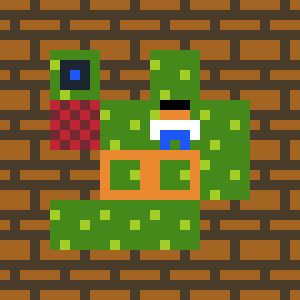
\includegraphics[width=0.25\textwidth]{Images/lavaGame}
    \caption{Example level from LavaGame showing the new metric}
    \label{Figure:lavaGame}
\end{figure}

\subsubsection{Heuristic Measures}
Heuristic measures are calculated using a weighted function of six measures.
\begin{itemize}
	\item \emph{Playing Score ($P_{score}$):} Playing score is used to ensure level playability. Based on the work by Nielsen et al.\cite{gvgpPerformanceProfiles}, a float value is assigned for how much the level is near the solution from the initial state. The Playing Score can be expressed by the following equation:
	\begin{center}$ P_{score} = S_{play} - S_{nothing}$\end{center}
	where $S_{play}$ is the automated player score and $S_{nothing}$ is the initial level score.
	
	\item\emph{Solution Length Score ($L_{score}$):} Since bigger levels needs longer solution, a score is given to the ratio between the solution length and the level area. We analyzed 40 hand crafted levels with different area from 5 different games. A histogram is plotted for the ratio and shown in \figref{solutionLengthHistogram}. The histogram seems to follow a Normal Distribution with $\mu = 1.221$ and $\sigma = 0.461$. Based on that, the Solution Length Score is expressed by the following equation:
	\begin{center}$L_{score} = Normal(\dfrac{L}{A}, 1.221, 0.461)$\end{center}
	where $Normal(ratio, \mu, \sigma)$ is a normal distribution function, $L$ is the solution length, and $A$ is the level area.
	\begin{figure}[ht]
		\centering
		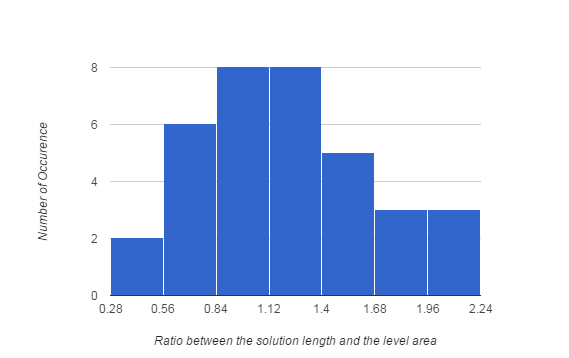
\includegraphics[width=0.5\textwidth]{Images/solutionLengthHistogram}
		\caption{Histogram for the ratio between the solution length and the level area}
		\label{Figure:solutionLengthHistogram}
	\end{figure}
	
	\item \emph{Object Number Score ($N_{score}$):} The Object Number Score is calculated by the following equation:
	\begin{center}$N_{score} = 0.4 * N_{rule} + 0.3 * N_{player} + 0.3 * N_{winning}$\end{center}
	\begin{itemize}
		\item \emph{Number of Rule Objects ($N_{rule}$):} is a score for the number of objects appearing in the level. An object is considered in the level if it appears greater than or equal to its minimum number property to ensure the possibility of applying every rule.
		\item \emph{Number of Players ($N_{player}$):} is a score for the number of players in the level. Generated levels should only have only one player.
		\item \emph{Number of Winning Objects ($N_{winning}$):} is a score for the number of winning objects in the level. This score ensures the number of the winning objects are equal, unless one of the winning objects have a Create behavior.
	\end{itemize}
	
	\item \emph{Box Line Score ($B_{score}$):} It is similar to Taylor and Parberry metric\cite{sokobanLevelGenerationNew} used in finding the farthest state. This metric calculates the number of unrepeated moves found in the solution and divide it by the solution length. The following equation represents it:
	\begin{center}$B_{score} = \dfrac{L_{unique}}{L}$\end{center}
	where $L_{unique}$ is the number of unrepeated moves in the solution and $L$ is the solution length.
	
	\item \emph{Applied Rule Score ($R_{score}$):} The ratio between the number of applied rules to the solution length is used to indicate good level design. To find the best ratio, we analyzed 40 hand crafted levels from 5 different games and a histogram is plotted in \figref{rulesSolutionLengthHistogram}. The histogram seems to follow a Normal Distribution with $\mu = 0.417$ and $\sigma = 0.128$. Based on that the Applied Rule Score can be expressed by the following equation:
	\begin{center}$R_{score} = Normal(\dfrac{R_{app} \pm R_{none}}{L}, 0.417, 0.128)$\end{center}
	where $Normal(ration, \mu, \sigma)$ is a normal distribution function, $R_{app}$ is the number of applied rules, $R_{none}$ is the number of applied rules without any previous actions, and $L$ is the solution length.
	\begin{figure}[ht]
		\centering
		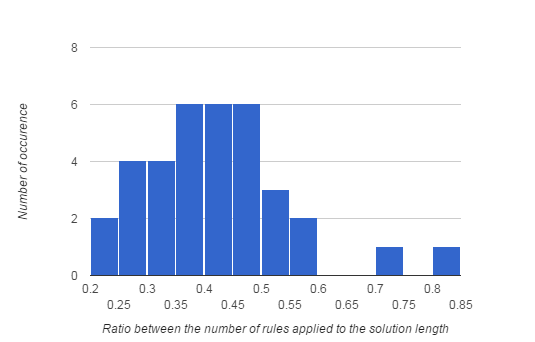
\includegraphics[width=0.5\textwidth]{Images/rulesSolutionLengthHistogram}
		\caption{Histogram for the number of rules applied to the solution length}
		\label{Figure:rulesSolutionLengthHistogram}
	\end{figure}
	
	\item \emph{Exploration Score ($E_{score}$):} The increase in the number of explored states by the automated player means that the current level is not obvious to be solved directly by the automated player heuristics. The following equation express this idea:
	\begin{center}
	$E_{score}= \begin{cases}
	               0.75 + \dfrac{N_{exp}}{N_{max}} & \text{solution exists}\\
	               0.5 & \text{no solution, }N_{exp} = N_{max}\\
	               0 & \text{no solution, }N_{exp} < N_{max}
	           \end{cases}$
	\end{center}
	where $N_{exp}$ is the number of explored states and $N_{max}$ is the maximum number of states the automated player can explore.
\end{itemize}

\section{Results and Evaluation}
The generated levels are published on our website \footnote{\url{http://www.amidos-games.com/puzzlescript-pcg/}} to collect human feedbacks. The following subsection analyzes the results of the new automated player and compares its results with the original one proposed in Lim et al. work\cite{puzzleScriptGeneration}, followed by the results of the level generation techniques and comparing it with human feedbacks.

\subsection{Tested Games}
Our system is tested against five games. The five games are completely different to cover different object behaviors and different winning conditions. These games are:
\begin{itemize} \itemsep0pt \parskip0pt \parsep0pt
	\item \emph{Sokoban:} The goal of the game is to place every single crate over a certain position. Player can push crates to achieve that goal.
	\item \emph{LavaGame:} The goal of the game is to reach the exit. The path towards the exit is always blocked by a lava. Player should push crates over the lava to clear his way.
	\item \emph{BlockFaker:} The goal of the game is to reach the exit. The path towards the exit is always blocked by lots of crates. Player should push these crates to align them vertically or horizontally. Every three aligned crates are destroyed which clear the path towards the exit.
	\item \emph{GemGame:} The goal of the game is to place at least one gem over one of several locations. Player can create gems by pushing crates. Every three aligned crates are replaced with a single gem instead of the middle crate.
	\item \emph{DestroyGame:} The goal of the game is to clear every single gem. Gems can be destroyed when they are aligned with two other crates vertically or horizontally. Player should push crates to reach that goal.
\end{itemize}

\subsection{Automated Player}
Forty handcrafted levels from the five games were used to compare the new player with the original one. Levels are designed with different sizes and ideas to cover different design aspects. Both players play all the forty levels and reports the solution length and the number of states explored. \figref{automatedPlayerPerformance} shows the average number of states each player explores in each game to reach the goal. The new player outperforms the original player in Sokoban and GemGame, but its almost the similar in the rest of the games. The new players performed badly in DestroyGame and LavaGame due to the presence of the Destroy behavior as the core mechanic of the game.\\\par

\begin{figure}[ht]
  	\centering
    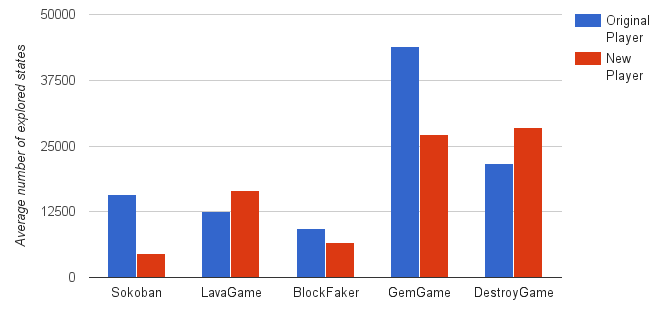
\includegraphics[width=0.5\textwidth]{Images/automatedPlayerPerformance}
    \caption{Comparison between the number of explored states for different automated players}
    \label{Figure:automatedPlayerPerformance}
\end{figure}

\figref{automatedPlayerLength} shows the average solution length for each game for the both players. The new player produces  a slightly shorter solutions than the original player. Comparing both \figref{automatedPlayerPerformance} and \figref{automatedPlayerLength} a correlation can be noticed between both of them except for Sokoban. Sokoban does not follow the same pattern due to being an abstract game. Sokoban has a very small amount of objects and just one rule. This abstraction is the main reason for both players reaching the goal in almost the same amount of steps.

\begin{figure}[ht]
  	\centering
    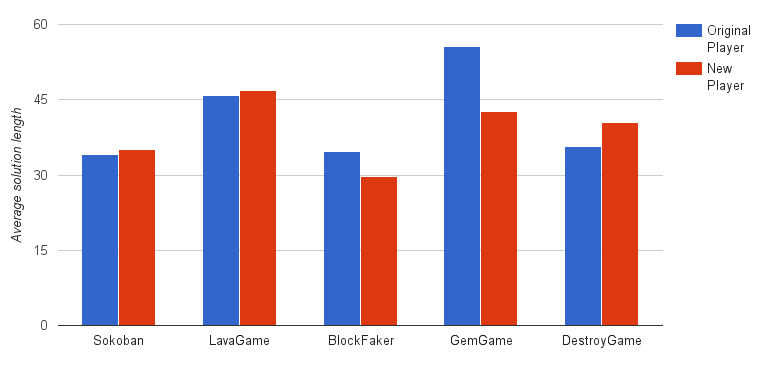
\includegraphics[width=0.5\textwidth]{Images/automatedPlayerLength}
    \caption{Comparison between the average solution length for different automated players}
    \label{Figure:automatedPlayerLength}
\end{figure}

\subsection{Level Generation}
This section shows the results of the level generation techniques. The new automated player is used with a limit of 5000 explored states to ensure fast execution. Level generation is tested against several level layouts to cover different sizes and inner structures. \figref{levelLayouts} shows the eight different level layouts used in generation.\\\par
\begin{figure}[ht]
  	\centering
    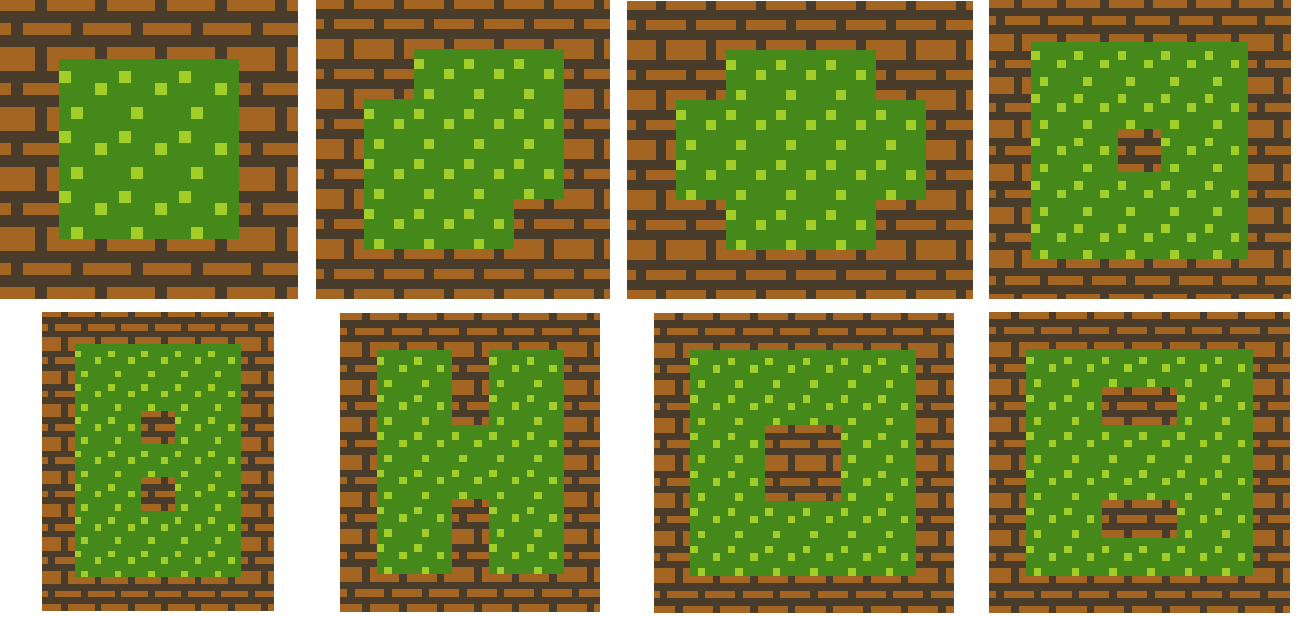
\includegraphics[width=0.45\textwidth]{Images/levelLayouts}
    \caption{Different level layouts for level generation}
    \label{Figure:levelLayouts}
\end{figure}

Scores from all the following techniques are combined and compared to human feedback. \figref{totalCorrelation} shows the correlation between system scores and human scores for all levels. The figure shows a good correlation between them. The reason for not having a very high correlation is due to the small amount of collected data and the presence of different ideas about a good level.

\begin{figure}[ht]
  	\centering
    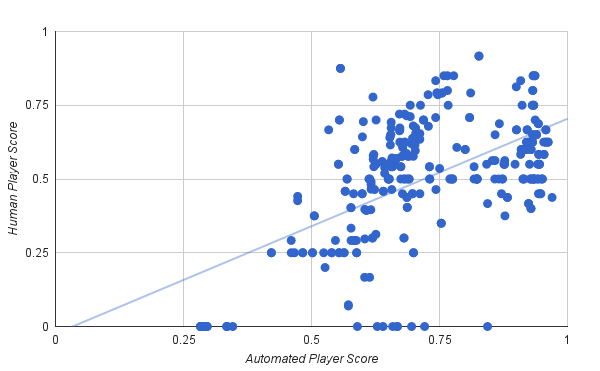
\includegraphics[width=0.45\textwidth]{Images/totalCorrelation}
    \caption{Correlation between automated player scores and human scores for all games}
    \label{Figure:totalCorrelation}
\end{figure}

\subsubsection{Constructive Approach}
One hundred levels are generated using the CA for each level layout. Each level is evaluated and the best two levels are selected. Out of the 80 selected levels only 15\% are reported as unplayable by the system. By testing these levels by human players only 10\% are completely unplayable while the remaining levels are very difficult levels to be solved by the automated player.

\subsubsection{Genetic Approach}
GA is used for 20 generations with a population equal to 50 chromosomes for each layout. The crossover rate is around 70\% and the mutation rate is around 10\%. GA is applied on each level layout and the best two chromosomes from each layout are selected. Elitism is used with probability equals to 2\%.
\begin{itemize}
	\item \emph{Random Initialization:} Out of the 80 selected levels only 75\% of them are playable although the automated player reported only 73.75\%.
	\item \emph{Constructive Initialization:} Using CA to initialize the GA increase the overall level playability from 90\% to reach 100\% by tuning the unplayable levels from the constructive approach.
	\item \emph{Mixed Initialization:} Same like constructive initialization with 100\% playability but with more diversity.
\end{itemize}

\subsubsection{Fitness Comparison}
The following figures show a comparison between the max fitness of the all presented techniques for Sokoban(\figref{sokobanComparison}), LavaGame(\figref{lavaGameComparisonmparison}), and BlockFaker(\figref{blockFakerComparison}). GA with constructive initialization has the highest score in almost all games, followed by GA with mixed initialization which is almost the same as GA with constructive initialization. The worst of them all is the GA with random initialization as it needs more generations to find a good playable levels. Sokoban scores in \figref{sokobanComparison} is almost similar with all techniques due to the simplicity of the game rules and the small number of objects needed to generate a playable level.

\begin{figure}[ht]
  	\centering
    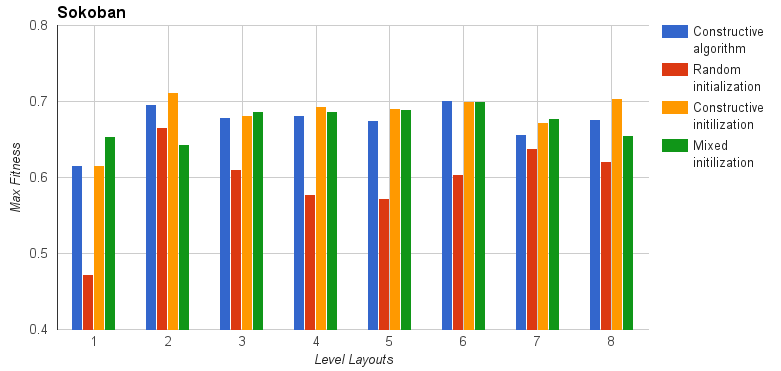
\includegraphics[width=0.5\textwidth]{Images/sokobanComparison}
    \caption{Max fitness of all proposed techniques for Sokoban}
    \label{Figure:sokobanComparison}
\end{figure}

\begin{figure}[ht]
  	\centering
    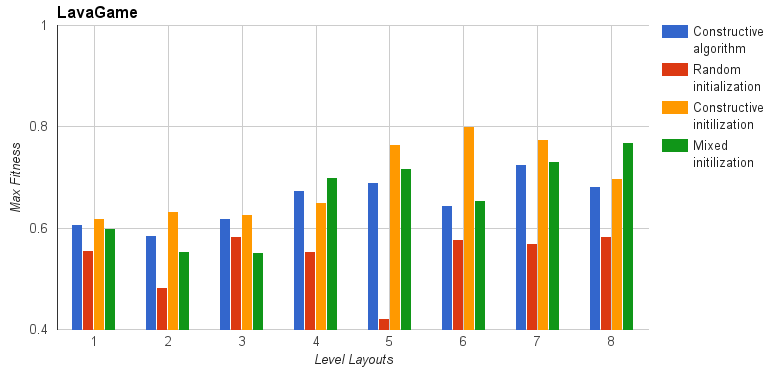
\includegraphics[width=0.5\textwidth]{Images/lavaGameComparison}
    \caption{Max fitness of all proposed techniques for LavaGame}
    \label{Figure:lavaGameComparisonmparison}
\end{figure}

\begin{figure}[ht]
  	\centering
    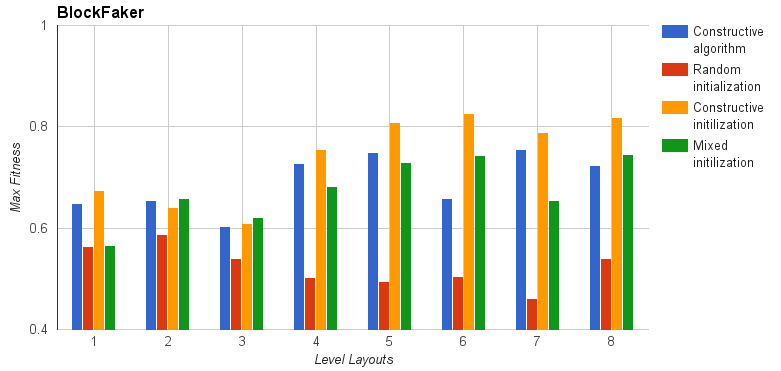
\includegraphics[width=0.5\textwidth]{Images/blockFakerComparison}
    \caption{Max fitness of all proposed techniques for BlockFaker}
    \label{Figure:blockFakerComparison}
\end{figure}

\section{Conclusion and Future Work}
This research presented a system to generate levels for Puzzle Script. Also, it proposed several metrics to evaluate puzzle levels based on their solution sequence.\\\par

The proposed system generates levels regardless of the game rules. It uses two different techniques (Constructive and Genetic approach). The constructive approach resulted in 90\% playable levels which is enhanced in the genetic approach to reach 100\% with more time. Genetic approach uses GA with three different initialization methods (Random initialization, Constructive initialization, and Mixed initialization). Random initialization produces levels with different configuration from the constructive approach, but with a low playability equals to 75\%.  The constructive approach produces levels with playability reaching 100\%, but with similar structure to the constructive approach. The mixed initialization is similar to the constructive initialization in terms of playability and it finds more diverse levels as well, but it needs more time to get better fitness than constructive initialization.\\\par

The generated levels are tested using human players and a score is given for each level. Comparing human scores with system scores shows a high correlation. This high correlation is a good indication that the proposed metrics can actually measure level's playability and challenge. The correlation is higher in some games such as BlockFaker and Sokoban due to the high performance of the automated player in playing them.\\\par

This work is a first stone in general level generation field. There is a plenty to be done to expand and enhance it. As for future work, we aim to:
\begin{itemize}
	\item analyze the effect of each metric on the generation techniques.
	\item utilize the metrics to analyze the search space for the generation techniques.
	\item test different techniques rather than plan GA to increase the level diversity like in Sorenson and Pasquier work\cite{genericLevelFramework}.
	\item improve the time and the quality of the automated player to decrease the generation time.
	\item generate levels with a specific difficulty.
\end{itemize}

\section{Acknowledgments}
I would like to express my deepest gratitude to Micheal Cook. His wok on ANGELINA was my main inspiration to start working on PCG. I would like to thank my supervisor Prof. Magda Fayek for all the support, guidance, and extreme patience she provides. Without her support this work would not have seen the light. Also Thanks to all my friends for the support and the huge help in collecting feedbacks on the results.

\bibliographystyle{iccc}
\bibliography{iccc}

\end{document}